%%%%%%%%%%%%%%%%%%%%%%%%%%%%%%%%%%%%%%%%%%%%%%%%%%%%%%%%%%%%%%%%%%%%%%%%%%
\documentclass[twocolumns,10pt,a4j]{jarticle}
%%%%%%%%%%%%%%%%%%%%%%%%%%%%%%%%%%%%%%%%%%%%%%%%%%%%%%%%%%%%%%%%%%%%%%%%%%
\usepackage{amsmath}
\usepackage[dvipdfmx]{graphicx}% Include figure files
%\usepackage{txfonts}
\usepackage{setspace}
\usepackage{bm}% bold math
\usepackage{here}
\usepackage{array}
\usepackage[T1]{fontenc}
\usepackage{etoolbox}
\usepackage[top=10truemm,bottom=25truemm,left=25truemm,right=20truemm]{geometry}%余白
\usepackage{layout}
\usepackage{wrapfig}
\renewcommand{\abstractname}{} 
\renewcommand{\figurename}{\small{Fig.}}
\renewcommand{\thefootnote}{\fnsymbol{footnote}}
\renewcommand{\baselinestretch}{0.80}
\usepackage{indentfirst}
\usepackage{otf}
%\usepackage{multicol}
\pagestyle{empty}
%%%%%%%%%%%%%%%%%%%%%%%%%%%%%%%%%%%%%%%%%%%%%%%%%%%%%%%%%%%%%%%%%%%%%%%%%%
\makeatletter%% プリアンブルで定義する場合は必須
\patchcmd{\maketitle}{\@fnsymbol}{\@alph}{}{}  % Footnote numbers from symbols to small letters
\long\def\@makecaption#1#2{% \@makecaption を再定義します
  \vskip\abovecaptionskip
  \iftdir\sbox\@tempboxa{#1\hskip1zw#2}%
  \else\sbox\@tempboxa{#1~ #2}% ここの : を ~ に変更する
  \fi
  \ifdim \wd\@tempboxa >\hsize% 
  \iftdir #1\hskip1zw#2\relax\par
  \else #1~ #2\relax\par\fi% ここの : を ~ に変更する
  \else
  \global \@minipagefalse
  \hbox to\hsize{\hfil\box\@tempboxa\hfil}% センタリング
  %   \hbox to\hsize{\box\@tempboxa\hfil}%      左詰め
  %   \hbox to\hsize{\hfil\box\@tempboxa}%      右詰め
  \fi
  \vskip\belowcaptionskip}

  \DeclareRobustCommand\cite{\unskip
  \@ifnextchar[{\@tempswatrue\@citex}{\@tempswafalse\@citex[]}}
  \def\@cite#1#2{$^{[\hbox{\scriptsize{#1\if@tempswa ,#2\fi}]}}$}
  \def\@biblabel#1{[#1]}
  \makeatother%% プリアンブルで定義する場合は必須
  \setlength{\columnsep}{8  truemm}
  \setlength{\linewidth}{81 truemm}
  %%%%%%%%%%%%%%%%%%%%%%%%%%%%%%%%%%%%%%%%%%%%%%%%%%%%%%%%%%%%%%%%%%%%%%
  \title{\Large せん断場でのマイクロスイマーのダイナミクス\vspace{-3truemm}}
  \author{\large 化学プロセス工学コース 移動現象論分野 荊尾太雅\vspace{-10zh}}
  \date{}
  %%%%%%%%%%%%%%%%%%%%%%%%%%%%%%%%%%%%%%%%%%%%%%%%%%%%%%%%%%%%%%%%%%%%%%
  \begin{document}

  %% start abstract

  \twocolumn[
    \maketitle\thispagestyle{empty}
    \vspace{-10truemm}
    \begin{quote}
      \normalsize
マイクロスイマーとは,バクテリアのように流体中を自己推進する微小な物体の総称である.
工学的にも応用性に富んでいるが,それらの集団運動を予測し制御するためには複雑な流体力学的相互作用を考慮する必要があり,未だに理解が進んでいない.
本研究ではsquirmerモデルを用いた直接数値計算を行い,せん断場での挙動を調べた.
    \end{quote}
  ]

  %% end abstract
  %% start 1.緒言

  \noindent
  {\bf \large 1.緒言}
  \par
マイクロスイマーの拘束空間内における集団的な動的挙動を理解することは,バイオフィルムの形成の説明や標的薬物送達システムの設計などの工学的な用途に有用である.
単成分系マイクロスイマーの動的挙動については解析されており,特にPuller型は拘束空間内において進行波のように特徴的な集団運動を示すことが判明している\cite{1}.
本研究では,直接数値計算を用いて,拘束空間内におけるPuller型/Pusher型2成分系の挙動を調べることを目的とした.

  %% end 1.
  %% start 2.計算手法

  \noindent
  {\bf \large 2.計算手法}
  \par
マイクロスイマーのモデルとして,squirmerモデルを採用した.このモデルでは,球状粒子で異なる泳動形態を表現するために,粒子表面において粒子と流体の速度差が式\eqref{boundary_I}で表される境界条件を用いる\cite{1}.

  \vspace{-3truemm}
    \begin{equation}
      \boldsymbol{u}^s = B_1\left(\sin{\theta} + \frac{\alpha}{2}\sin{2\theta}\right)\hat{\boldsymbol{\theta}}
      \label{boundary_I}
    \end{equation}
  \vspace{-4truemm}

  \noindent
ここで,$\boldsymbol{u}^s$はスイマー表面の流れ場,$B_1$はフーリエ級数の係数第1項,$\alpha$はスイマーのタイプを与える定数,
$\theta$は動径ベクトルと推進方向との間の極角,$\hat{\boldsymbol{\theta}}$は単位極角ベクトルである.
$\alpha<0$では推進方向に伸張流場を生成するPusher型,$\alpha=0$で潜在的な流れ場で泳ぐNeutral型,$\alpha>0$で推進方向に収縮流場を生成するPuller型を示す(Fig.\ref{squirmer})\cite{1}.
  % \vspace{-3truemm}
  % \begin{figure}[H]
  %   \centering
  %   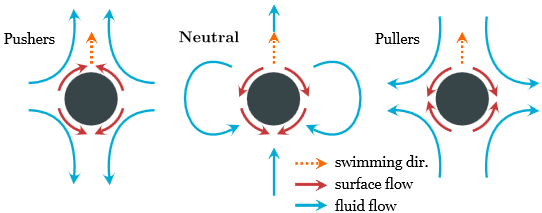
\includegraphics[width=7cm]{./images/squirmer_2.png}
  %   \vspace{-4truemm}
  %   \caption{Schematic representation of the squirmer model}
  %   \label{squirmer}
  % \end{figure}
  % \vspace{-4truemm}

直接数値計算は,squirmerモデルをSPMに組み込んで行った.
SPMは流体力学を用いた固体/流体2相ダイナミクス問題の効率的な計算方法である\cite{2}.
流体の支配方程式として非圧縮性流体におけるNavier-Stokes方程式を用い,スイマーの時間発展はNewton-Euler方程式(\ref{Newton_Euler})で与える.

  \par
1.Navier-Stokes方程式\\
  \vspace{-6truemm}
  \begin{equation}
    \begin{split}
      \boldsymbol{\nabla}\cdot\boldsymbol{u}&=0 \\
      \rho_{\rm f}\left(\partial_t+\boldsymbol{u}\cdot\boldsymbol{\nabla}\right)\boldsymbol{u}&=\boldsymbol{\nabla}\cdot\boldsymbol{\sigma}+\rho_{\rm f}\left(\phi_{\rm p}\boldsymbol{f}_{\rm p}+\boldsymbol{f}_{\rm sq}\right)
    \end{split}
    \label{Navier_Stokes}
  \end{equation}
  \vspace{-4truemm}

  \noindent
ここで,$\boldsymbol u $は全速度場,$\rho_{\rm f}$は流体の質量密度,$t$は時間,$\boldsymbol{\sigma}$は応力テンソル,$\phi_{\rm p}$は[0,1]の値を連続的に持つ界面関数,$\phi_{\rm p}\boldsymbol{f}_{\rm p}$は粒子の剛直性を保証する体積力,$\boldsymbol{f}_{\rm sq}$は流体との速度差を生じる力である.
  \par
2.Newton-Euler方程式\\
  \vspace{-6truemm}
  \begin{equation}
    \begin{split}
      &\quad\dot{\boldsymbol{R}}_i = \boldsymbol{V}_i
      \quad ,\quad
      \dot{\boldsymbol{Q}}_i = \text{skew}(\boldsymbol{\Omega}_i)\cdot \boldsymbol{Q}_i,\\
      &M_{\text{p}}\dot{\boldsymbol{V}}_i = \boldsymbol{F}_i^{\text{H}}+\boldsymbol{F}_i^{\text{C}}
      \quad ,\quad
      \boldsymbol{I}_{\text{p}}\cdot\dot{\boldsymbol{\Omega}}_i = \boldsymbol{N}_i^{\text{H}}
    \end{split}
    \label{Newton_Euler}
  \end{equation}
  \vspace{-4truemm}

  \noindent
ここでスイマー$i$について,$\boldsymbol{R}_i$は位置,$\boldsymbol{V}_i$は速度,$\boldsymbol{\Omega}_i$は角速度を示す.$\boldsymbol{Q}_i$は回転行列, $M_{\rm p}$はスイマーの質量,$\boldsymbol{F}_i^{\text{H}}$は流体力,$\boldsymbol{F}_i^{\text{C}}$は粒子間直接的相互作用による力,$\boldsymbol{I}_{\text{p}}$は慣性モーメント,$\boldsymbol{N}_i^{\text{H}}$はトルクである.

  %% end 2.
  %% start 3.結果と考察

  \noindent
  {\bf \large 3.結果と考察}
  \par
直径$4\Delta$,$\alpha\pm0.5$のsquirmerについて,体積分率を0.13として$64\Delta×\!\!160\Delta×\!\!64\Delta$の矩形システムでシミュレーションを行った.
このシステムは$x$方向と$z$方向には周期的であるが,$y$方向には$y =1\Delta$と$y=159\Delta$の位置に配置された球状粒子の平行壁に挟まれている(Fig.\ref{Confinement_model}).
ここで,$\Delta$は格子間隔と単位長さである.また,Puller型/Pusher型2成分の組成比を変えて計算を行った場合の局所密度の時間発展をFig.\ref{wave}に示す.

  % \vspace{-2mm}
  % \begin{figure}[h]
  %   \begin{tabular}{cc}
  %     \hspace{-3mm}
  %     \begin{minipage}[t]{0.44\hsize}
  %       \centering
  %       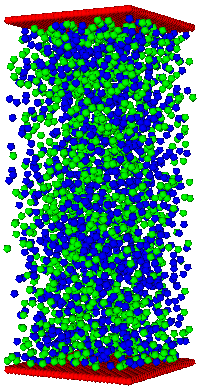
\includegraphics[width=24mm]{./images/Confinement_model.png}
  %       \vspace{-4mm}
  %       \hspace{-2mm}
  %       \caption{Simulation snapshot}
  %       \label{Confinement_model}
  %     \end{minipage}

  %     \hspace{2mm}
  %     \vspace{-2mm}
  %     \begin{minipage}[t]{0.44\hsize}
  %       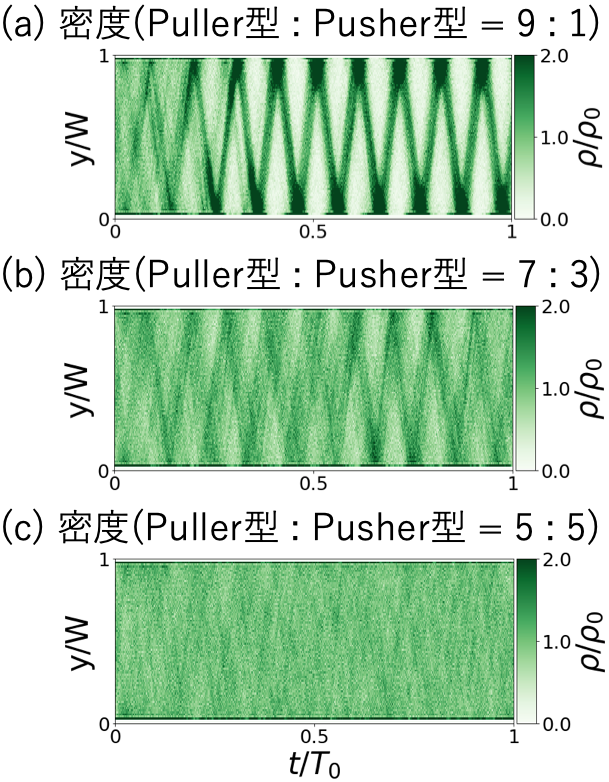
\includegraphics[width=37mm]{./images/wave.png}
  %       \vspace{-10mm}
  %       \caption{Time evolution of local density}
  %       \label{wave}
  %     \end{minipage}
  %     \vspace{-1mm}
  %   \end{tabular}
  % \end{figure}

  \noindent
ここで,$W(=160\Delta)$は$y$方向のシステムサイズ,$T_0$は全計算時間,$\rho$は局所密度,$\rho_0$は平均密度である.
Fig.\ref{wave}より,拘束空間内におけるPuller型の分率が高いほど,より進行波が明確に発生することが確認できた.
そして,Puller型の分率が低くなるにつれて進行波の発生は抑制され,次第に進行波の発生が確認できなくなることも確認された.
Puller型の分率が高いときは同方向に推進するPuller型の個体数も多く,そのためPuller型が運動するに従って生じる推進方向への収縮流場の影響を多大に受けて互いに引き付け合うことが,
squirmer全体が疎密波のような集団運動を引き起こす要因になるのではないかと考えられる.


  %% end 3.
  %% start 4.結言

  \noindent
  \textbf{\large 4.結言}
  \par
マイクロスイマーのモデルにsquirmerモデルを採用し,平行壁に挟まれた矩形システムの中でマイクロスイマー2成分系の局所密度の時間発展の解析を行った.
その結果,Puller型の分率が多いほどシステム内における疎密波の形成傾向が強まることを定量的に示した.
  \vspace{-7.5truemm}

  %% end 4.
  %% start 参考文献

  \renewcommand{\refname}{\normalsize 参考文献\vspace{-3truemm}}
  \begin{thebibliography}{9}
  %
  \bibitem{1}
    N. Oyama,博士論文,(2017).\\
  %
  \vspace{-7truemm}
  %
  \bibitem{2}
    Y. Nakayama,K. Kim,and R. Yamamoto,\textit{The European Physical Journal E},\textbf{26},361-368 (2008).\\
  %
  \end{thebibliography}

  %% end 参考文献
  %% satrt 締め

  \vspace{-7truemm}
  \centering
  \underline{指導教員名\hspace{10truemm} 山本 量一 \hspace{20truemm} 印}

  %% end 締め

\end{document}
